% Created 2025-10-15 Wed 10:54
% Intended LaTeX compiler: pdflatex
\documentclass[11pt]{article}
\usepackage[utf8]{inputenc}
\usepackage[T1]{fontenc}
\usepackage{graphicx}
\usepackage{longtable}
\usepackage{wrapfig}
\usepackage{rotating}
\usepackage[normalem]{ulem}
\usepackage{amsmath}
\usepackage{amssymb}
\usepackage{capt-of}
\usepackage{hyperref}
\author{PA156562}
\date{\today}
\title{}
\hypersetup{
 pdfauthor={PA156562},
 pdftitle={},
 pdfkeywords={},
 pdfsubject={},
 pdfcreator={},
 pdflang={English}}

% Setup for code blocks [1/2]

\usepackage{fvextra}

\fvset{%
  commandchars=\\\{\},
  highlightcolor=white!95!black!80!blue,
  breaklines=true,
  breaksymbol=\color{white!60!black}\tiny\ensuremath{\hookrightarrow}}

% Make line numbers smaller and grey.
\renewcommand\theFancyVerbLine{\footnotesize\color{black!40!white}\arabic{FancyVerbLine}}

\usepackage{xcolor}

% In case engrave-faces-latex-gen-preamble has not been run.
\providecolor{EfD}{HTML}{f7f7f7}
\providecolor{EFD}{HTML}{28292e}

% Define a Code environment to prettily wrap the fontified code.
\usepackage[breakable,xparse]{tcolorbox}
\DeclareTColorBox[]{Code}{o}%
{colback=EfD!98!EFD, colframe=EfD!95!EFD,
  fontupper=\footnotesize\setlength{\fboxsep}{0pt},
  colupper=EFD,
  IfNoValueTF={#1}%
  {boxsep=2pt, arc=2.5pt, outer arc=2.5pt,
    boxrule=0.5pt, left=2pt}%
  {boxsep=2.5pt, arc=0pt, outer arc=0pt,
    boxrule=0pt, leftrule=1.5pt, left=0.5pt},
  right=2pt, top=1pt, bottom=0.5pt,
  breakable}

% Support listings with captions
\usepackage{float}
\floatstyle{plain}
\newfloat{listing}{htbp}{lst}
\newcommand{\listingsname}{Listing}
\floatname{listing}{\listingsname}
\newcommand{\listoflistingsname}{List of Listings}
\providecommand{\listoflistings}{\listof{listing}{\listoflistingsname}}


% Setup for code blocks [2/2]: syntax highlighting colors

\newcommand\efstrut{\vrule height 2.1ex depth 0.8ex width 0pt}
\definecolor{EFD}{HTML}{000000}
\definecolor{EfD}{HTML}{ffffff}
\newcommand{\EFD}[1]{\textcolor{EFD}{#1}} % default
\definecolor{EFvp}{HTML}{000000}
\newcommand{\EFvp}[1]{\textcolor{EFvp}{#1}} % variable-pitch
\definecolor{EFh}{HTML}{7f7f7f}
\newcommand{\EFh}[1]{\textcolor{EFh}{#1}} % shadow
\definecolor{EFsc}{HTML}{228b22}
\newcommand{\EFsc}[1]{\textcolor{EFsc}{\textbf{#1}}} % success
\definecolor{EFw}{HTML}{ff8e00}
\newcommand{\EFw}[1]{\textcolor{EFw}{\textbf{#1}}} % warning
\definecolor{EFe}{HTML}{ff0000}
\newcommand{\EFe}[1]{\textcolor{EFe}{\textbf{#1}}} % error
\definecolor{EFl}{HTML}{ff0000}
\newcommand{\EFl}[1]{\textcolor{EFl}{#1}} % link
\definecolor{EFlv}{HTML}{ff0000}
\newcommand{\EFlv}[1]{\textcolor{EFlv}{#1}} % link-visited
\definecolor{EFhi}{HTML}{ff0000}
\newcommand{\EFhi}[1]{\textcolor{EFhi}{#1}} % highlight
\definecolor{EFc}{HTML}{b22222}
\newcommand{\EFc}[1]{\textcolor{EFc}{#1}} % font-lock-comment-face
\definecolor{EFcd}{HTML}{b22222}
\newcommand{\EFcd}[1]{\textcolor{EFcd}{#1}} % font-lock-comment-delimiter-face
\definecolor{EFs}{HTML}{8b2252}
\newcommand{\EFs}[1]{\textcolor{EFs}{#1}} % font-lock-string-face
\definecolor{EFd}{HTML}{8b2252}
\newcommand{\EFd}[1]{\textcolor{EFd}{#1}} % font-lock-doc-face
\definecolor{EFm}{HTML}{008b8b}
\newcommand{\EFm}[1]{\textcolor{EFm}{#1}} % font-lock-doc-markup-face
\definecolor{EFk}{HTML}{9370db}
\newcommand{\EFk}[1]{\textcolor{EFk}{#1}} % font-lock-keyword-face
\definecolor{EFb}{HTML}{483d8b}
\newcommand{\EFb}[1]{\textcolor{EFb}{#1}} % font-lock-builtin-face
\definecolor{EFf}{HTML}{0000ff}
\newcommand{\EFf}[1]{\textcolor{EFf}{#1}} % font-lock-function-name-face
\definecolor{EFv}{HTML}{a0522d}
\newcommand{\EFv}[1]{\textcolor{EFv}{#1}} % font-lock-variable-name-face
\definecolor{EFt}{HTML}{228b22}
\newcommand{\EFt}[1]{\textcolor{EFt}{#1}} % font-lock-type-face
\definecolor{EFo}{HTML}{008b8b}
\newcommand{\EFo}[1]{\textcolor{EFo}{#1}} % font-lock-constant-face
\definecolor{EFwr}{HTML}{ff0000}
\newcommand{\EFwr}[1]{\textcolor{EFwr}{\textbf{#1}}} % font-lock-warning-face
\newcommand{\EFnc}[1]{#1} % font-lock-negation-char-face
\definecolor{EFpp}{HTML}{483d8b}
\newcommand{\EFpp}[1]{\textcolor{EFpp}{#1}} % font-lock-preprocessor-face
\newcommand{\EFrc}[1]{\textbf{#1}} % font-lock-regexp-grouping-construct
\newcommand{\EFrb}[1]{\textbf{#1}} % font-lock-regexp-grouping-backslash
\newcommand{\EFob}[1]{#1} % org-block
\newcommand{\EFobb}[1]{#1} % org-block-begin-line
\newcommand{\EFobe}[1]{#1} % org-block-end-line
\definecolor{EFOa}{HTML}{0000ff}
\newcommand{\EFOa}[1]{\textcolor{EFOa}{#1}} % outline-1
\definecolor{EFOb}{HTML}{a0522d}
\newcommand{\EFOb}[1]{\textcolor{EFOb}{#1}} % outline-2
\definecolor{EFOc}{HTML}{a020f0}
\newcommand{\EFOc}[1]{\textcolor{EFOc}{#1}} % outline-3
\definecolor{EFOd}{HTML}{b22222}
\newcommand{\EFOd}[1]{\textcolor{EFOd}{#1}} % outline-4
\definecolor{EFOe}{HTML}{228b22}
\newcommand{\EFOe}[1]{\textcolor{EFOe}{#1}} % outline-5
\definecolor{EFOf}{HTML}{008b8b}
\newcommand{\EFOf}[1]{\textcolor{EFOf}{#1}} % outline-6
\definecolor{EFOg}{HTML}{483d8b}
\newcommand{\EFOg}[1]{\textcolor{EFOg}{#1}} % outline-7
\definecolor{EFOh}{HTML}{8b2252}
\newcommand{\EFOh}[1]{\textcolor{EFOh}{#1}} % outline-8
\definecolor{EFhn}{HTML}{008b8b}
\newcommand{\EFhn}[1]{\textcolor{EFhn}{#1}} % highlight-numbers-number
\definecolor{EFhq}{HTML}{9370db}
\newcommand{\EFhq}[1]{\textcolor{EFhq}{#1}} % highlight-quoted-quote
\definecolor{EFhs}{HTML}{008b8b}
\newcommand{\EFhs}[1]{\textcolor{EFhs}{#1}} % highlight-quoted-symbol
\definecolor{EFrda}{HTML}{707183}
\newcommand{\EFrda}[1]{\textcolor{EFrda}{#1}} % rainbow-delimiters-depth-1-face
\definecolor{EFrdb}{HTML}{7388d6}
\newcommand{\EFrdb}[1]{\textcolor{EFrdb}{#1}} % rainbow-delimiters-depth-2-face
\definecolor{EFrdc}{HTML}{909183}
\newcommand{\EFrdc}[1]{\textcolor{EFrdc}{#1}} % rainbow-delimiters-depth-3-face
\definecolor{EFrdd}{HTML}{709870}
\newcommand{\EFrdd}[1]{\textcolor{EFrdd}{#1}} % rainbow-delimiters-depth-4-face
\definecolor{EFrde}{HTML}{907373}
\newcommand{\EFrde}[1]{\textcolor{EFrde}{#1}} % rainbow-delimiters-depth-5-face
\definecolor{EFrdf}{HTML}{6276ba}
\newcommand{\EFrdf}[1]{\textcolor{EFrdf}{#1}} % rainbow-delimiters-depth-6-face
\definecolor{EFrdg}{HTML}{858580}
\newcommand{\EFrdg}[1]{\textcolor{EFrdg}{#1}} % rainbow-delimiters-depth-7-face
\definecolor{EFrdh}{HTML}{80a880}
\newcommand{\EFrdh}[1]{\textcolor{EFrdh}{#1}} % rainbow-delimiters-depth-8-face
\definecolor{EFrdi}{HTML}{887070}
\newcommand{\EFrdi}[1]{\textcolor{EFrdi}{#1}} % rainbow-delimiters-depth-9-face
\definecolor{EFany}{HTML}{CDCD00}
\newcommand{\EFany}[1]{\textcolor{EFany}{#1}} % ansi-color-yellow
\definecolor{EFanr}{HTML}{CD0000}
\newcommand{\EFanr}[1]{\textcolor{EFanr}{#1}} % ansi-color-red
\definecolor{EFanb}{HTML}{000000}
\newcommand{\EFanb}[1]{\textcolor{EFanb}{#1}} % ansi-color-black
\definecolor{EFang}{HTML}{00CD00}
\newcommand{\EFang}[1]{\textcolor{EFang}{#1}} % ansi-color-green
\definecolor{EFanB}{HTML}{0000EE}
\newcommand{\EFanB}[1]{\textcolor{EFanB}{#1}} % ansi-color-blue
\definecolor{EFanc}{HTML}{00CDCD}
\newcommand{\EFanc}[1]{\textcolor{EFanc}{#1}} % ansi-color-cyan
\definecolor{EFanw}{HTML}{E5E5E5}
\newcommand{\EFanw}[1]{\textcolor{EFanw}{#1}} % ansi-color-white
\definecolor{EFanm}{HTML}{CD00CD}
\newcommand{\EFanm}[1]{\textcolor{EFanm}{#1}} % ansi-color-magenta
\definecolor{EFANy}{HTML}{EEEE00}
\newcommand{\EFANy}[1]{\textcolor{EFANy}{#1}} % ansi-color-bright-yellow
\definecolor{EFANr}{HTML}{EE0000}
\newcommand{\EFANr}[1]{\textcolor{EFANr}{#1}} % ansi-color-bright-red
\newcommand{\EFANb}[1]{#1} % ansi-color-bright-black
\definecolor{EFANg}{HTML}{00EE00}
\newcommand{\EFANg}[1]{\textcolor{EFANg}{#1}} % ansi-color-bright-green
\definecolor{EFANB}{HTML}{0000FF}
\newcommand{\EFANB}[1]{\textcolor{EFANB}{#1}} % ansi-color-bright-blue
\definecolor{EFANc}{HTML}{00EEEE}
\newcommand{\EFANc}[1]{\textcolor{EFANc}{#1}} % ansi-color-bright-cyan
\newcommand{\EFANw}[1]{#1} % ansi-color-bright-white
\newcommand{\EFANm}[1]{#1} % ansi-color-bright-magenta
\begin{document}

\tableofcontents

\section{Introduction}
\label{sec:org6dbc753}

\subsection{Background}
\label{sec:orgcf4b5a5}
\subsection{Business rules}
\label{sec:orgc1ae20d}

\subsection{Ecological interface design}
\label{sec:org161dbf9}
\section{Protocol de recherche}
\label{sec:org74f7c68}
\subsection{Questions de recherche}
\label{sec:org8993bea}
Questions principales
\begin{description}
\item[{\label{orgb3cdbf5}RQ1}] Comment les principes de l’Ecological Interface Design ont-ils été appliqués à la représentation visuelle de règles métiers ou de systèmes de contraintes ?
\item[{\label{orga5f2884}RQ2}] Quelles approches conceptuelles, méthodologiques ou techniques ont été mobilisées pour rendre visibles ou compréhensibles les états d’une règle métier (valide, bloquée, inactive, en alerte, etc.) ?
\item[{\label{org552f46f}RQ3}] Quels modèles cognitifs, ergonomiques ou informationnels ont été mobilisés pour adapter la visualisation des règles métiers au contexte d’usage (rôle utilisateur, environnement, phase de travail, niveau d’expertise, etc.) ?
\end{description}

Questions secondaires
\begin{description}
\item[{\label{orgaa71ef6}RQ4}] Quels types de métaphores visuelles ou structures d’information ont été proposés pour représenter la complexité des interdépendances entre règles métiers (hiérarchie, causalité, propagation d’état) ?
\item[{\label{org1ee453a}RQ5}] Quels domaines applicatifs ont le plus exploré ces approches (ex. : systèmes industriels, ingénierie, santé, finance, administration, etc.) et dans quelles finalités (supervision, décision, audit, apprentissage) ?
\item[{\label{orgacde9b6}RQ6}] Quelles sont les limites identifiées dans la littérature concernant l’applicabilité des principes EID à des systèmes de règles dynamiques (ex. : règles générées, apprises, modifiées en temps réel) ?
\item[{\label{org922a236}RQ7}] Quels modèles d’évaluation (performance, charge cognitive, compréhension, décision) ont été employés pour mesurer l’efficacité de ces interfaces écologiques appliquées aux règles métiers ?
\end{description}



inline [rmq::some remq] remarque. \footnote{text}

\begin{longtable}{|p{3cm}|p{5cm}|p{7cm}|}
\caption{\label{tab:org64ddc88}Methode PICOC}
\\
\hline
Element & Definition & Keywords\\
\hline
\endfirsthead
\multicolumn{3}{l}{Continued from previous page} \\
\hline

Element & Definition & Keywords \\

\hline
\endhead
\hline\multicolumn{3}{r}{Continued on next page} \\
\endfoot
\endlastfoot
\hline
\textbf{\textbf{Population}} &  & \\
\textbf{\textbf{Intervention}} &  & \texttt{ecological interface design}, \texttt{EID}\\
\textbf{\textbf{Comparison}} & Non utilisé & \\
\textbf{\textbf{Outcome}} &  & \\
\textbf{\textbf{Context}} &  & \\
\hline
\end{longtable}
\subsubsection{Quality assessment criteria}
\label{sec:orgdfa250d}
Justification des choix de mots-clés.

L'identification des mots clés permet de préparer la requête des bases de données. Le processus de collecte est illustré par la figure \ref{fig:org071c30a}.

\begin{figure}[htbp]
\centering
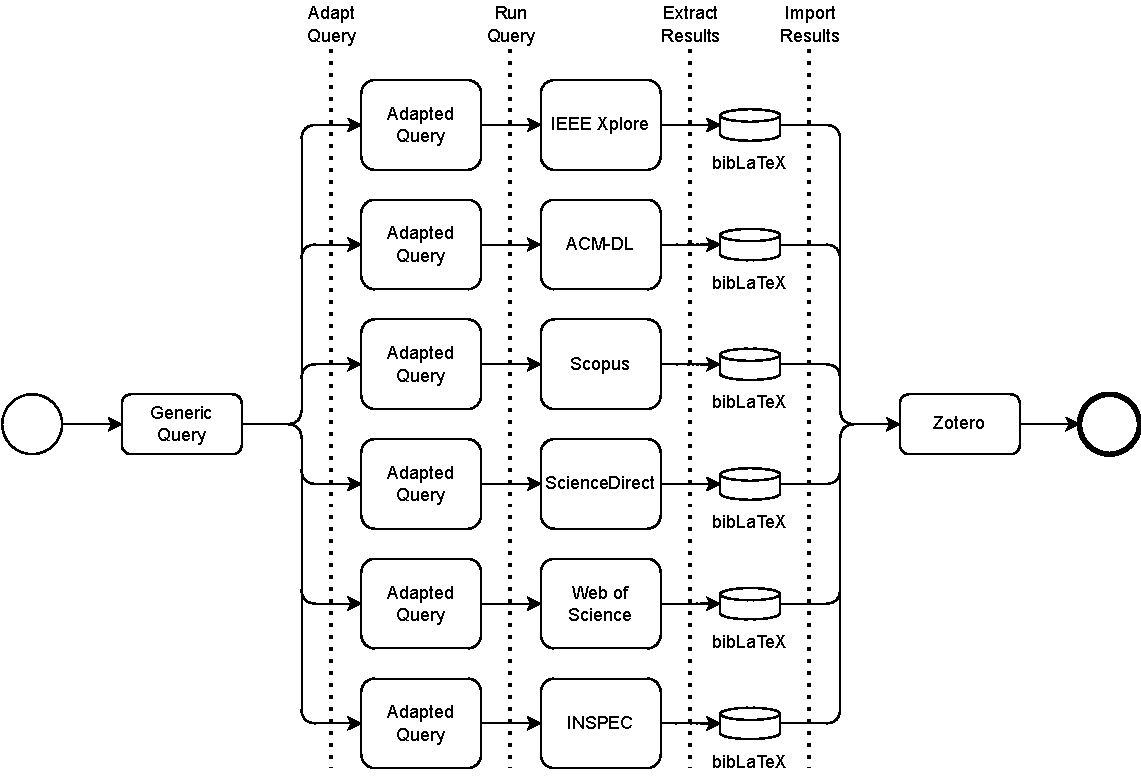
\includegraphics[width=.9\linewidth]{./svg/slr-data-collect.pdf}
\caption{\label{fig:org071c30a}Processus de collecte des données}
\end{figure}

La requête booléenne générique intégrant les mots-clés issus du tableau \ref{tab:org64ddc88} est présentée par le bloc de code \ref{lst:org887aa52}. Sa structure suit l’ordre logique : \textbf{Population \(\land\) Intervention \(\land\) Outcome \(\land\) Context}.

\begin{listing}[htbp]
\begin{Code}
\begin{Verbatim}
\color{EFD}\EFcd{--} \EFc{POPULATION: Interfaces, cognition, visualization}
("human-machine interface" \EFk{OR} "human computer interaction" \EFk{OR} "human centered interaction" \EFk{OR} "HMI" \EFk{OR} "HCI")
\EFcd{--} \EFc{INTERVENTION: Ecological Interface Design}
\EFk{AND} ("ecological interface design" \EFk{OR} "EID")
\EFcd{--} \EFc{OUTCOME: cognitive and decision-related outcomes}
\EFk{AND} ("situational awareness" \EFk{OR} "context sensitivity" \EFk{OR} "cognitive load" \EFk{OR} "usability" \EFk{OR} "mental workload" \EFk{OR} "\EFb{user} performance" \EFk{OR} "task performance" \EFk{OR} "error reduction" \EFk{OR} "cognitive efficiency")
\EFcd{--} \EFc{CONTEXT: construction and engineering disciplines}
\EFk{AND} ("construction industry" \EFk{OR} "civil" \EFk{OR} "structural" \EFk{OR} "geotechnical" \EFk{OR} "hydraulic" \EFk{OR} "transport" \EFk{OR} "mechanical" \EFk{OR} "plumbing" \EFk{OR} "sanitary" \EFk{OR} "HVAC"  \EFk{OR} "heating" \EFk{OR} "ventilation" \EFk{OR} "air conditioning" \EFk{OR} "cooling" \EFk{OR} "climate" \EFk{OR} "environmental" \EFk{OR} "electrical" \EFk{OR} "power" \EFk{OR} "energy" \EFk{OR} "lighting" \EFk{OR} "acoustical" \EFk{OR} "thermal" \EFk{OR} "fire safety" \EFk{OR} "industrial" \EFk{OR} "maintenance" \EFk{OR} "construction management" \EFk{OR} "urban" \EFk{OR} "infrastructure")
\end{Verbatim}
\end{Code}
\caption{\label{lst:org887aa52}Requête générique}
\end{listing}

Les bases de données intérogées sont :
\begin{enumerate}
\item IEEE Xplore
\item ACM Digital Library : The ACM Guide to Computing Literature collection
\item Scopus
\item ScienceDirect
\item Web of Science
\item INSPEC (via Engineering Village or ProQuest)
\end{enumerate}

La requête générique est ainsi adaptée à chaque base de données et les variantes sont présentées par le tableau \ref{tab:org7aeac38}

\begin{longtable}{|p{3cm}|p{12cm}|"}
\caption{\label{tab:org7aeac38}Déclinaison de la requête générique par bases de données ciblées}
\\
\hline
Base de données & Requête\\
\hline
\endfirsthead
\multicolumn{2}{l}{Continued from previous page} \\
\hline

Base de données & Requête \\

\hline
\endhead
\hline\multicolumn{2}{r}{Continued on next page} \\
\endfoot
\endlastfoot
\hline
IEEE Xplore & \Small{"All Metadata":(("human-machine interface" OR "human computer interaction" OR "HMI" OR "HCI") AND ("ecological interface design" OR "EID" OR "ecological design") AND ("situational awareness" OR "context sensitivity" OR "cognitive load" OR "usability" OR "mental workload" OR "user performance" OR "task performance" OR "error reduction" OR "cognitive efficiency") AND (("construction industry" OR "civil engineering" OR "structural engineering" OR "geotechnical engineering" OR "hydraulic engineering" OR "transport engineering" OR "mechanical engineering" OR "plumbing" OR "sanitary engineering" OR "HVAC" OR "heating ventilation air conditioning" OR "climate engineering" OR "environmental engineering" OR "electrical engineering" OR "power engineering" OR "energy engineering" OR "lighting engineering" OR "building physics" OR "acoustical engineering" OR "thermal engineering" OR "fire safety engineering" OR "industrial engineering" OR "maintenance engineering" OR "construction management" OR "architecture" OR "urban engineering" OR "public works" OR "infrastructure engineering")))}\\
\hline
ACM-DL & \Small{("human-machine interface" OR "human computer interaction" OR "HMI" OR "HCI") AND ("ecological interface design" OR "EID" OR "ecological design") AND ("situational awareness" OR "context sensitivity" OR "cognitive load" OR "usability" OR "mental workload" OR "user performance" OR "task performance" OR "error reduction" OR "cognitive efficiency") AND ("construction industry" OR "civil engineering" OR "structural engineering" OR "geotechnical engineering" OR "hydraulic engineering" OR "transport engineering" OR "mechanical engineering" OR "plumbing" OR "sanitary engineering" OR "HVAC" OR "heating ventilation air conditioning" OR "climate engineering" OR "environmental engineering" OR "electrical engineering" OR "power engineering" OR "energy engineering" OR "lighting engineering" OR "building physics" OR "acoustical engineering" OR "thermal engineering" OR "fire safety engineering" OR "industrial engineering" OR "maintenance engineering" OR "construction management" OR "architecture" OR "urban engineering" OR "public works" OR "infrastructure engineering")}\\
\hline
Scopus & \Small{TITLE-ABS-KEY(("human-machine interface" OR "human computer interaction" OR "HMI" OR "HCI") AND ("ecological interface design" OR "EID" OR "ecological design") AND ("situational awareness" OR "context sensitivity" OR "cognitive load" OR "usability" OR "mental workload" OR "user performance" OR "task performance" OR "error reduction" OR "cognitive efficiency") AND (("construction industry" OR "civil engineering" OR "structural engineering" OR "geotechnical engineering" OR "hydraulic engineering" OR "transport engineering" OR "mechanical engineering" OR "plumbing" OR "sanitary engineering" OR "HVAC" OR "heating ventilation air conditioning" OR "climate engineering" OR "environmental engineering" OR "electrical engineering" OR "power engineering" OR "energy engineering" OR "lighting engineering" OR "building physics" OR "acoustical engineering" OR "thermal engineering" OR "fire safety engineering" OR "industrial engineering" OR "maintenance engineering" OR "construction management" OR "architecture" OR "urban engineering" OR "public works" OR "infrastructure engineering")))}\\
\hline
ScienceDirect & \Small{TITLE-ABS-KEY(("human-machine interface" OR "human computer interaction" OR "HMI" OR "HCI") AND ("ecological interface design" OR "EID" OR "ecological design") AND ("situational awareness" OR "context sensitivity" OR "cognitive load" OR "usability" OR "mental workload" OR "user performance" OR "task performance" OR "error reduction" OR "cognitive efficiency") AND (("construction industry" OR "civil engineering" OR "structural engineering" OR "geotechnical engineering" OR "hydraulic engineering" OR "transport engineering" OR "mechanical engineering" OR "plumbing" OR "sanitary engineering" OR "HVAC" OR "heating ventilation air conditioning" OR "climate engineering" OR "environmental engineering" OR "electrical engineering" OR "power engineering" OR "energy engineering" OR "lighting engineering" OR "building physics" OR "acoustical engineering" OR "thermal engineering" OR "fire safety engineering" OR "industrial engineering" OR "maintenance engineering" OR "construction management" OR "architecture" OR "urban engineering" OR "public works" OR "infrastructure engineering")))}\\
\hline
Web of Science & \Small{TS=(("human-machine interface" OR "human computer interaction" OR "HMI" OR "HCI") AND ("ecological interface design" OR "EID" OR "ecological design") AND ("situational awareness" OR "context sensitivity" OR "cognitive load" OR "usability" OR "mental workload" OR "user performance" OR "task performance" OR "error reduction" OR "cognitive efficiency") AND (("construction industry" OR "civil engineering" OR "structural engineering" OR "geotechnical engineering" OR "hydraulic engineering" OR "transport engineering" OR "mechanical engineering" OR "plumbing" OR "sanitary engineering" OR "HVAC" OR "heating ventilation air conditioning" OR "climate engineering" OR "environmental engineering" OR "electrical engineering" OR "power engineering" OR "energy engineering" OR "lighting engineering" OR "building physics" OR "acoustical engineering" OR "thermal engineering" OR "fire safety engineering" OR "industrial engineering" OR "maintenance engineering" OR "construction management" OR "architecture" OR "urban engineering" OR "public works" OR "infrastructure engineering")))}\\
\hline
INSPEC & \Small{(TI=("human-machine interface" OR "human computer interaction" OR "HMI" OR "HCI")) AND (TI=("ecological interface design" OR "EID" OR "ecological design")) AND (TI=("situational awareness" OR "context sensitivity" OR "cognitive load" OR "usability" OR "mental workload" OR "user performance" OR "task performance" OR "error reduction" OR "cognitive efficiency") OR AB=("situational awareness" OR "context sensitivity" OR "cognitive load" OR "usability" OR "mental workload" OR "user performance" OR "task performance" OR "error reduction" OR "cognitive efficiency")) AND (TI=("construction industry" OR "civil engineering" OR "structural engineering" OR "geotechnical engineering" OR "hydraulic engineering" OR "transport engineering" OR "mechanical engineering" OR "plumbing" OR "sanitary engineering" OR "HVAC" OR "heating ventilation air conditioning" OR "climate engineering" OR "environmental engineering" OR "electrical engineering" OR "power engineering" OR "energy engineering" OR "lighting engineering" OR "building physics" OR "acoustical engineering" OR "thermal engineering" OR "fire safety engineering" OR "industrial engineering" OR "maintenance engineering" OR "construction management" OR "architecture" OR "urban engineering" OR "public works" OR "infrastructure engineering") OR AB=("construction industry" OR "civil engineering" OR "structural engineering" OR "geotechnical engineering" OR "hydraulic engineering" OR "transport engineering" OR "mechanical engineering" OR "plumbing" OR "sanitary engineering" OR "HVAC" OR "heating ventilation air conditioning" OR "climate engineering" OR "environmental engineering" OR "electrical engineering" OR "power engineering" OR "energy engineering" OR "lighting engineering" OR "building physics" OR "acoustical engineering" OR "thermal engineering" OR "fire safety engineering" OR "industrial engineering" OR "maintenance engineering" OR "construction management" OR "architecture" OR "urban engineering" OR "public works" OR "infrastructure engineering"))}\\
\hline
\end{longtable}

Nous limitons la collecte d'articles à une profondeur de 10 ans soit entre le 2015-01-01 et le 2025-01-01. Seuls les articles de revues et de colloque en anglais, associés à l'interraction humain-machine sont retenus.
Nous écartons les articles non revues par les pairs, les articles incomplets et ceux sans résultats empiriques.
L'opération de déduplication est réalisée sur Zotero.
\subsection{Processus de recherche}
\label{sec:org896f22c}
Recherche initiale → collecte des résultats → exportation (BibTeX, CSV).
Déduplication (Zotero, EndNote, Mendeley, etc.).

Les articles sont préparés puis sélectionnés en suivant le processus présenté en figure [[ .
Automatique (Action tag, plugin, etc.)
\begin{description}
\item[{Etape 1}] Déduplication \texttt{(merge-entries (:where (= :DOI :Title)))}
\item[{Etape 2}] Filtration \texttt{(delete-entries (:where (and (< :date "2015-01-01") (not (= :langue "en")))))}
\end{description}

Mannuel systématique
\begin{description}
\item[{Etape 3}] non revues par les pairs, incomplets, sans résultats empiriques.
\end{description}

Mannuel collégial
\begin{description}
\item[{Étape 4}] filtrage par titre et résumé.
\item[{Étape 5}] filtrage par texte intégral.
\item[{Étape 3}] validation inter-évaluateurs (au moins deux chercheurs).
\end{description}
\subsection{Formulaire d’extraction}
\label{sec:org0df211d}
Champs obligatoires :
    Identifiant (ID)
    Référence bibliographique complète
    Année de publication
    Contexte (population, domaine, technologie)
    Méthodologie de l’étude
    Résultats principaux (Outcome)
    Limites rapportées
\subsection{Évaluation de la qualité}
\label{sec:org1f1546c}
Checklist PRISMA, indiquer la localisation de chaque item dans le rapport final.

Checklist qualité (exemple) :
    Clarté des objectifs : oui/non
    Méthodologie décrite : oui/non
    Données empiriques disponibles : oui/non
    Validité des résultats : élevé/moyen/faible
\subsection{Schéma de sélection}
\label{sec:org2a6a5ac}
Nombre d’articles identifiés, filtrés, exclus, inclus.

\textbf{PRISMA 2020 flow diagram} for new systematic reviews which included searches of databases and registers only
\section{Analysis and results}
\label{sec:org7535351}
Méthodes d’analyse
    Quantitative (comptages, distributions, tendances temporelles).
    Qualitative (analyse thématique, catégorisation, taxonomie).
    Meta-analysis (si applicable).
\section{Wrapping up}
\label{sec:org651f08d}
\subsection{General discussion}
\label{sec:org6b12b93}
Contribution scientifique :
    Lacunes identifiées
    Etat de l’art consolidé.
Contribution pratique :
    Recommandations
    Implications pour les chercheurs et praticiens.
Limites méthodologiques du protocole.
\subsection{Recommendations}
\label{sec:org997fc70}
\section{Treats to validity}
\label{sec:org45a3380}
Risques de biais de publication.
Risques liés à l’échantillonnage ou aux bases de données.
Stratégies d’atténuation (diversification, double codage).
\section{Research opportunity}
\label{sec:org58a076b}

\section{Conclusion}
\label{sec:org9282ece}
\end{document}
